\begin{frame}[plain]
	\centering
	\begin{tikzpicture}
		\node[draw, minimum width=3.5cm, minimum height=2.5cm] (framework) at (0,0) {\Large \textbf{Framework}};

		\node[] (task) at (-3.8,1.3) {\Large \textbf{Planning Task}};
		\node[] (task2) at (-4.5,2.3) {
\includegraphics[scale=0.05]{images/rover1.png}};
		\node[] (task3) at (-3.1,2.3) {
\includegraphics[scale=0.05]{images/rover2.png}};
		\node[] (task4) at (-4.5,3.3) {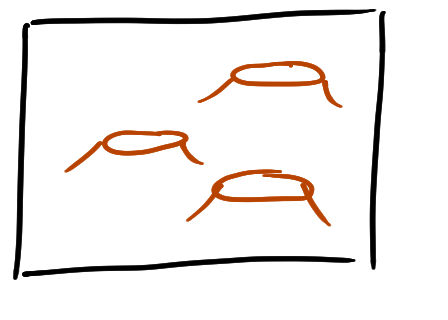
\includegraphics[scale=0.05]{images/image1.png}};
		\node[] (task5) at (-3.85,3.3) {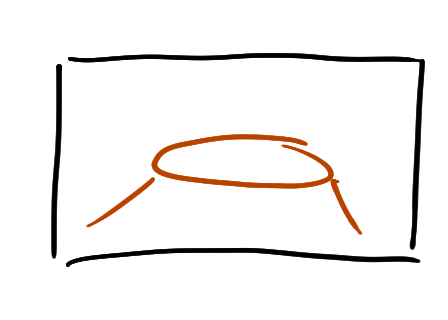
\includegraphics[scale=0.05]{images/image2.png}};
		\node[] (task6) at (-3.1,3.3) {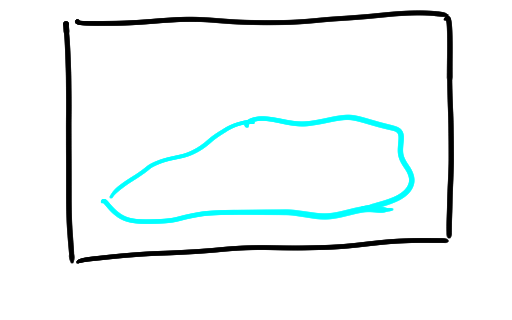
\includegraphics[scale=0.05]{images/image3.png}};

		\node[] (props) at (-3.8,-1.1) {\Large \textbf{Properties}};
		\node[draw, inner sep=1pt] (props1) at (-4.6,-2.5) {
			\resizebox{!}{1.2cm}{%
				\dontuseconnection{1}{1}{2}
			}
		};
		\node[draw, inner sep=1pt] (props2) at (-2.8,-2.5) {
			\resizebox{!}{1.2cm}{%
				\specificrover{1}{1}
			}
		};

		%\node[] (no) at (-3.8,-1.8) {
\includegraphics[scale=0.3]{images/no.png}};

		\node[] (plan) at (3.8,1.3) {\Large \textbf{Plan}};
		\node[draw, align=left, fill=white] (plan2) at (4,3.0) {
				\scriptsize
				$drive(R_1,L_1,L2)$\\[-0.2cm]
				\scriptsize
				$takeImage_1(R_1)$\\[-0.2cm]
				\scriptsize
				$drive(R_2,L_4,L_5)$\\[-0.2cm]
				\scriptsize
				$takeImage_3(R_2)$\\[-0.2cm]
				\scriptsize
				$drive(R_2,L_5,L_6)$\\[-0.2cm]
				\scriptsize
				$\cdots$
		};

		\node[] (exp) at (3.8,-1.3) {\Large \textbf{Explanation}};
		\node[] (exp2) at (3.8,-2.5) {
			\resizebox{!}{1cm}{%
			\begin{tikzpicture}
				\node[draw] (p1) at (5,0) {
					\specificrover{1}{1}
				};

				\node[draw] (p4) at (0,0) {
					\dontuseconnection{1}{1}{2}
				};
				\node[] (not) at (5,0) {
\includegraphics[scale=0.3]{images/no.png}};

				\draw[thick, ->] (p4) to (p1);
			\end{tikzpicture}
			}
		};

		\draw[->, line width=2pt] (-4,0) to (-2.5,0);
		\draw[->, line width=2pt] (2.5,0) to (4,0);

	\end{tikzpicture}

\end{frame}



